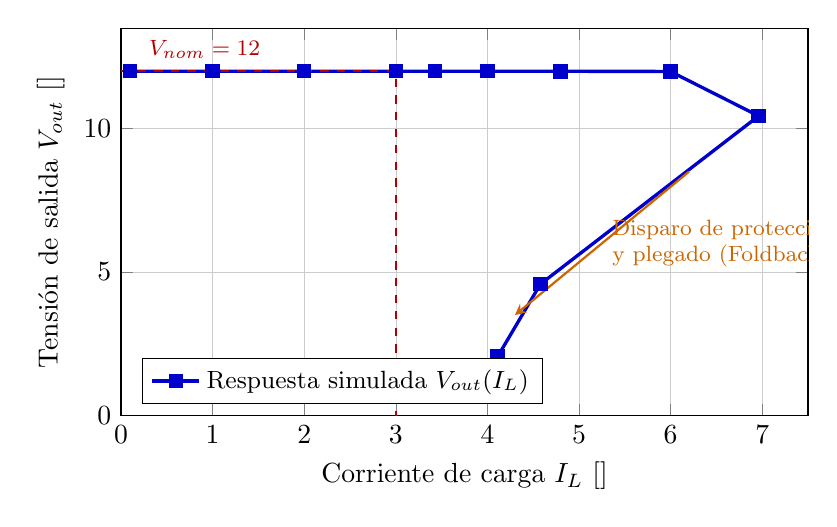
\begin{tikzpicture}
\begin{axis}[
    width=0.85\textwidth,
    height=6.5cm,
    xlabel={Corriente de carga $I_L$ [\si{\ampere}]},
    ylabel={Tensión de salida $V_{out}$ [\si{\volt}]},
    grid=both,
    grid style={line width=.1pt, draw=gray!20},
    major grid style={line width=.2pt, draw=gray!40},
    xmin=0, xmax=7.5,
    ymin=0, ymax=13.5,
    legend pos=south west,
    legend style={font=\small}
]

% Curva de salida Vo vs IL (comportamiento de tension constante y foldback)
\addplot[
    color=blue!80!black,
    mark=square*,
    mark size=2pt,
    line width=1.2pt
] coordinates {
    (0.100, 12.002)
    (1.000, 12.000)
    (2.000, 12.000)
    (3.000, 11.999)
    (3.428, 11.999)
    (4.000, 11.999)
    (4.799, 11.998)
    (5.997, 11.994)
    (6.961, 10.442)
    (4.578, 4.578)
    (4.112, 2.056)
};
\addlegendentry{Respuesta simulada $V_{out}(I_L)$}

% Linea de referencia nominal
\addplot[dashed, color=red!70!black, line width=0.8pt] coordinates {
    (0, 12) (3, 12) (3, 0)
};
\node[anchor=south west, text=red!70!black, font=\footnotesize] at (axis cs: 0.2, 12.1) {$V_{nom} = \SI{12}{\volt}$};
\node[anchor=south, text=red!70!black, font=\footnotesize] at (axis cs: 3.0, 0.2) {$I_{Lmax} = \SI{3}{\ampere}$};

% Anotacion de zona de foldback / corto
\draw[->, >=stealth, line width=0.8pt, color=orange!80!black] 
    (axis cs: 6.2, 8.5) -- (axis cs: 4.3, 3.5) 
    node[midway, right, font=\footnotesize, align=left] {Disparo de protección\\y plegado (Foldback)};

\end{axis}
\end{tikzpicture}
